%\documentstyle[epsf,twocolumn]{jarticle}       %LaTeX2e仕様
%\documentclass[twocolumn]{jarticle}     %pLaTeX2e仕様(platex.exeの場合)
\documentclass[onecolumn]{ujarticle}   %pLaTeX2e仕様(uplatex.exeの場合)
%%%%%%%%%%%%%%%%%%%%%%%%%%%%%%%%%%%%%%%%%%%%%%%%%%%%%%%%%%%%%%
%%
%%  基本バージョン
%%
%%%%%%%%%%%%%%%%%%%%%%%%%%%%%%%%%%%%%%%%%%%%%%%%%%%%%%%%%%%%%%%%
\setlength{\topmargin}{-45pt}
%\setlength{\oddsidemargin}{0cm} 
\setlength{\oddsidemargin}{-7.5mm}
%\setlength{\evensidemargin}{0cm} 
\setlength{\textheight}{24.1cm}
%setlength{\textheight}{25cm} 
\setlength{\textwidth}{17.4cm}
%\setlength{\textwidth}{172mm} 
\setlength{\columnsep}{11mm}

%\kanjiskip=.07zw plus.5pt minus.5pt


% 【節が変わるごとに (1.1)(1.2) … (2.1)(2.2) と数式番号をつけるとき】
%\makeatletter
%\renewcommand{\theequation}{%
%\thesection.\arabic{equation}} %\@addtoreset{equation}{section}
%\makeatother

%\renewcommand{\arraystretch}{0.95} 行間の設定
%%%%%%%%%%%%%%%%%%%%%%%%%%%%%%%%%%%%%%%%%%%%%%%%%%%%%%%%
%\usepackage{graphicx}   %pLaTeX2e仕様(\documentstyle ->\documentclass)
\usepackage[dvipdfmx]{graphicx}
\usepackage{subcaption}
\usepackage{multirow}
\usepackage{amsmath}
\usepackage{url}
\usepackage{ulem}
%%%%%%%%%%%%%%%%%%%%%%%%%%%%%%%%%%%%%%%%%%%%%%%%%%%%%%%%
\begin{document}
	
	%bibtex用の設定
	%\bibliographystyle{ujarticle} 
	\noindent
	
	\hspace{1em}
	2019 年 10 月 11 日
	ゼミ資料
	\hfill
	M1 寺内 光
	
	\vspace{2mm}
	
	\hrule
	
	\begin{center}
		{\Large \bf 進捗報告}
	\end{center}
	
	
	\hrule
	\vspace{3mm}
	
	% ‚ここから 文章 Start!
	\section{今週やったこと}
	\begin{itemize}
		\item ラベル画像をインデックスカラー画像として見れるようにした
		\item 一連の実験(training, evaluation, visualize)がオリジナルデータセットでできるようになった
	\end{itemize}

	\subsection{ラベル画像をインデックスカラー画像として見れるようにした}
	PILを用いてラベル画像をインデックス画像として扱えるようにした.すなわち画素的にはRGB(1, 1, 1)が入っているが表示の際にはカラーパレットマップと対応させることで(例えば)赤色に着色してみることができ,セマンティックセグメンテーションのタスクに関しては非常に有用な保存方法である.図\ref{fig:indexed}に例を示す.この画像にいては目の領域にRGBにそれぞれ1が入っている.今回はpascal\_vocのカラーパレットをそのまま利用した.図 \ref{fig:color_palette} にカラーパレットを示す.
	\begin{figure}[h]
		\centering
		\vspace{-7mm}
		\begin{subfigure}{0.45\columnwidth}
			\centering
			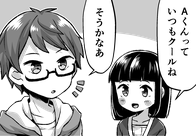
\includegraphics[width=1.3\columnwidth]{1_original.png}
			\caption{original}
		\end{subfigure}
		\begin{subfigure}{0.45\columnwidth}
			\centering
			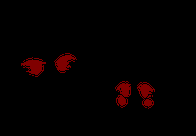
\includegraphics[width=1.3\columnwidth]{1_indexed.png}
			\caption{indexed}
		\end{subfigure}
		\caption{オリジナル画像とラベルのインデックスカラー画像}
		\label{fig:indexed}
	\end{figure}

	\begin{figure}[h]
		\centering
		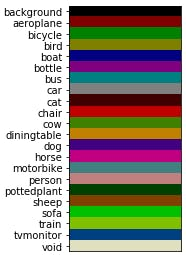
\includegraphics[width=0.8\columnwidth]{color_palette.jpg}
		\caption{pascal vocのカラーパレット(上からインデックスが0, 1, 2...のクラスを表す.)}
		\label{fig:color_palette}
	\end{figure}

	\subsection{一連の実験をまわすことができた}
	Tensorflowで実装されているDeeplabv3+のオリジナルデータセットに対する実験のエラー周りを片付けて(ほとんどこの作業をしていました)一通り回るようになった.

	\section{今後の課題}
	今後の課題としてはひとまずフル(240枚-目無し画像の枚数)のデータセットで回したいので来週を目途にデータセットの整形のシェルと変換のスクリプトを作成し,回し終わるところまでいきたい.

	
\end{document}